\documentclass[review]{elsarticle}

\usepackage{multirow}
\usepackage{lineno}
\usepackage{xspace}
\usepackage{threeparttable}
\usepackage{subfig}
\modulolinenumbers[5]

%% Journal name here
\journal{FIXME: The Journal Name Goes Here}

%% `Elsevier LaTeX' style
\bibliographystyle{elsarticle-num}
%%%%%%%%%%%%%%%%%%%%%%%

%%%% packages and definitions (optional)
\usepackage{placeins}
\usepackage{booktabs} % nice rules (thick lines) for tables
\usepackage{microtype} % improves typography for PDF
\usepackage{hhline}
\usepackage{amsmath}
\usepackage{subfig}

\usepackage{booktabs}
\usepackage{threeparttable, tablefootnote}

\usepackage{tabularx}

%% Special typesetting for Cyclus
\newcommand{\Cyclus}{\textsc{Cyclus}\xspace}%
\newcommand{\Cycamore}{\textsc{Cycamore}\xspace}%
\graphicspath{images/}

% tikz %
\usepackage{tikz}
\usetikzlibrary{positioning, arrows, decorations, shapes}

\usetikzlibrary{shapes.geometric,arrows}
\tikzstyle{process} = [rectangle, rounded corners, minimum width=3cm, minimum height=1cm,text centered, draw=black, fill=blue!30]
\tikzstyle{object} = [ellipse, rounded corners, minimum width=3cm, minimum height=1cm,text centered, draw=black, fill=green!30]
\tikzstyle{arrow} = [thick,->,>=stealth]

% hyperref %
\usepackage[hidelinks]{hyperref}
% after hyperref %
\usepackage{cleveref}
\usepackage{datatool}
\usepackage[acronym,toc]{glossaries}
\include{acros}

\makeglossaries

\begin{document}
\begin{frontmatter}
\title{FIXME: The Title Goes Here}

%\date{}                     % uncomment if you don't need date to appear

% Authors
\author[uiuc]{Jin Whan Bae}
\author[uiuc]{Clifford E. Singer}
\author[uiuc]{Kathryn D. Huff\corref{corrauthor}}
\cortext[corrauthor]{Corresponding Author}
\ead{kdhuff@illinois.edu}


% Institutes of the authors
\input{institutions}

\begin{keyword}
FIXME \sep
key words \sep
go here \sep
like: \sep 
simulation \sep
spent nuclear fuel 
\end{keyword}

\begin{abstract}
        The French 2012-2015 Commission Nationale d'Evaluation Reports
emphasize preparation for a transition from \glspl{LWR} to \glspl{SFR}.
We used the \Cyclus nuclear fuel cycle simulator to explore the feasibility of enabling a French
transition to an \gls{SFR} fleet by using \gls{UNF} from other \gls{EU} nations.
A \Cyclus simulation captured nuclear power deployment in the \gls{EU} from 
1970 to 2160. In this simulation, France begins its planned transition 
to \glspl{SFR} as existing \glspl{LWR} are decommissioned. These \glspl{SFR} 
are fuelled with \gls{UNF} accumulated by other \gls{EU} nations and 
reprocessed in France.
The impact of reactor lifetime extensions and \gls{SFR} breeding ratios on 
time-to-transition were investigated with additional simulations. 
These simulation demonstrates that France can avoid deployment of additional 
\glspl{LWR} by accepting \gls{UNF} from other EU nations, that lifetime 
extensions delay time-to-transition, and improved breeding ratios are not 
particularly impactful.
\end{abstract}



\end{frontmatter}
\glsresetall

%% Shows line numbers
\linenumbers

\section{Abstract}
The French 2012-2015 Commission Nationale d'Evaluation reports
\cite{noauthor_reports_2015} emphasize preparation for a transition from \glspl{LWR} to \glspl{SFR}.
This paper uses \Cyclus to explore the feasibility of using \gls{UNF} from other EU nations
for French transition into a \gls{SFR} fleet without additional construction of \glspl{LWR}.
A \Cyclus simulation ran from 1950 to 2160 for EU to track the \gls{UNF} mass
and tails inventory to support
the transition into \glspl{SFR}. Another simulation ran to model French
transition to \glspl{SFR} supported by reprocessing the \gls{UNF} inventory.
The study concludes that France can avoid deployment
of additional \glspl{LWR} by accepting \gls{UNF} from other EU nations.


\section{Introduction}
We used \Cyclus to analyze
the future nuclear inventory in the European Union. \Cyclus is an agent-based extensible
framework for modeling the flow of material through future nuclear cycles \cite{huff_fundamental_2016}.
This paper focuses on the used fuel
inventory in \gls{EU} member states in 2050, and focuses on a potential strategy of used fuel
management.
A major focus of this paper is to determine the extent to which France has an incentive
to receive all the \gls{UNF} from \gls{EU} nations to create \gls{MOX}.
The \gls{MOX} created will fuel French transition to a \gls{SFR} fleet
and allow France to avoid building additional \glspl{LWR}.

Past research, focused solely on France, typically assumes that additional \glspl{LWR},
namely \glspl{EPR} supply \gls{UNF} to produce \gls{MOX} \cite{carre_overview_2009, martin_symbiotic_2017, freynet_multiobjective_2016}.
Studies exist on implementation of partitioning and transmutation
in a regional (European) context, with \glspl{ADS} and Gen-IV reactors \cite{fazio_study_2013}.
There is little attention paid to reprocessing legacy \gls{UNF} from other
EU nations to produce \gls{MOX} for the newly deployed \glspl{SFR}.
The present work finds that this collaborative strategy can reduce the
need to construct additional \glspl{LWR} in France.

\section{Methodology}
The nuclear history of EU nations is modeled, using the \gls{PRIS} open-source 
database from \gls{IAEA}. That database is imported as a csv file, to populate the simulation
with deployment information, listing the country, reactor unit, type, net capacity (MWe), status,
operator, construction date, first criticality date, first grid date, commercial date, shutdown
date (if applicable), and unit capacity factor for 2013. Then only the \gls{EU} countries are extracted
from the csv file. A python script is written up to generate a \Cyclus input file from the csv file,
which lists the individual reactor units as agents. After running the \Cyclus input file,
another python script analyzes the output file. All the scripts and data used
in this paper are available in \cite{bae_arfc/transition-scenarios:_2017}.
%% Probably a separate repository is needed..?

Two \Cyclus simulations are run for this paper. 
The first simulation calculates
the mass and composition of used fuel and tails \gls{EU} nations accumulate from 1970 to 2050,
as well as the amount of \gls{MOX} that the \gls{UNF} inventory creates.
All EU nations with the exception of France adopts a once-through fuel cycle.
France can reprocess used \gls{UOX} and \gls{MOX} to
produce \gls{MOX} from reprocessed plutonium and depleted uranium (tails).

%%% PASSIVE PHRASE WHAT TO DO
After obtaining the \gls{UNF} inventory of all \gls{EU} in 2050, the second
simulation runs where the \gls{UNF} inventory is reprocessed and fabricated
as fuel for the newly deployed \gls{SFR} reactors.
\gls{SFR} per model after the ASTRID reactor.
ASTRID-type \glspl{SFR} make up for the decommissioned capacity
of \glspl{LWR} in France, to remain a constant installed capacity of $66,000$ MWe up to 2160.
It is assumed that ASTRID-type reactors use \gls{MOX} fuel created from 11\% reprocessed plutonium
and 89\% tails and burns the \gls{MOX} fuel to approximately 100 GWdth/t.
The high burnup allows breeding of plutonium.
Eventually, the  \gls{MOX} created from recycled \gls{MOX}
fuels the entire fleet of 110 \glspl{SFR}.


\subsection{Assumptions}
The paper makes the following assumptions:
\begin{itemize}
        \item \gls{SFR} technology is available for deployment in 2040.
        \item Decay is not taken into account.
        \item Reactor construction is always completed on time.
        \item Separated uranium is unused and stockpiled.
        \item \glspl{LWR} have an assumed lifetime of 60 years, unless shut down prematurely.
        \item Newly deployed \glspl{SFR} have a lifetime of 80 years.
        \item Additional assumptions in the \gls{SFR} case include:
        \begin{itemize}
        	\item Reprocessing and \gls{MOX} fabrication begins in 2020.
        	\item French nuclear capacity remains constant at 66,000 MWe.
        	\item Reprocessing and fabrication capacity is unlimited.
        \end{itemize}
\end{itemize}


\subsection{Deployment Timeline}
Projections of future reactor deployment in this simulation is based on assessment of analyses
from references such as \gls{PRIS} for reactors planned for construction \cite{iaea_pris_nodate},
the World Nuclear Association and two other papers for future plans in EU nations
\cite{world_nuclear_association_nuclear_2017, joskow_future_2012, hatch_politics_2015}.
The projections extend to 2050 at the latest. This allows the simulation to take place from
1970 to 2050, the latest foreseeable future. Later sections explain, in detail, the specific plans for each \gls{EU} nation.

Figure \ref{fig:eu_pow} displays the
timeseries of installed capacity in \gls{EU} nations.

\begin{figure}[htbp!]
	\begin{center}
		\includegraphics[scale=0.7]{./images/eu_future/power_plot.png}
	\end{center}
	\caption{Timeseries of installed nuclear capacity in \gls{EU}.}
	\label{fig:eu_pow}
\end{figure}
\FloatBarrier

\subsection{French \gls{SFR} Deployment Schedule}

Once \glspl{SFR} become available, in 2040,
600-MWe \glspl{SFR} are deployed to make up for the 
decommissioned \gls{LWR} capacities. 
This results in an installed capacity of 66,000 MWe
of \gls{SFR} by 2076, when the last \gls{LWR} decommissions.

\begin{figure}[htbp!]
        \begin{center}
                \includegraphics[scale=0.7]{./images/french-transition/power_plot.png}
        \end{center}
        \caption{French Transition into an SFR Fleet}
        \label{fig:sfr_num}
\end{figure}
\begin{figure}[htbp!]
	\begin{center}
		\includegraphics[scale=0.7]{./images/french-transition/sfr_deploy.png}
	\end{center}
	\caption{Deployment of French \glspl{SFR} and total installed capacity}
	\label{fig:dep}
\end{figure}
\FloatBarrier


\Cref{fig:sfr_num} and \cref{fig:dep} display
the French transition to \glspl{SFR} over time.
The steep transition from 2040 to 2060 reflects the scheduled
decommissioning of reactors built in the 1975-2000
era of aggressive nuclear growth in France.


\subsection{Material Definitions}
Depletion calculations of the nuclear fuel are recipe-based, such that a fresh 
and used fuel recipe is used for each reactor type.
For the compositions of the fuel, a reference depletion calculation
from ORIGEN is used (see \cref{tab:comp}). The recipe has also been used for
\cite{wilson_adoption_2009}.


\subsection{Scenario Descriptions}
The simulation follows the model fuel cycle, illustrated in \cref{diag:fc},
where a `source' provides natural uranium, which is enriched by an 'enrichment'
facility to produce \gls{UOX}, while disposing enrichment waste (tails)
to the 'sink' facility. The enriched \gls{UOX} fuels
the \gls{LWR}s and \gls{UOX} waste is produced. The used fuel
is sent to a pool to cool for 3 years \cite{carre_overview_2009}.
The cooled fuel is then reprocessed to separate plutonium and uranium,
or sent to a repository.
The plutonium mixed with depleted uranium (tails) makes \gls{MOX}.
The reprocessed uranium is unused and stockpiled. Uranium is reprocessed
in order to separate the raffinate (Minor actinides and fission products)
from 'usable' material. Though not utilized in this paper, reprocessed
uranium may substitute depleted uranium for \gls{MOX} production. In this
paper, there was sufficient depleted uranium inventory that using reprocessed
uranium was not considered. However, further in the future where the depleted
uranium inventory drains, reprocessed uranium (or, natural uranium) will need to be utilized. 


% Define block styles
\tikzstyle{decision} = [diamond, draw, fill=blue!20, 
text width=4.5em, text badly centered, node distance=3cm, inner sep=0pt]
\tikzstyle{block} = [rectangle, draw, fill=blue!20, 
text width=5em, text centered, rounded corners, minimum height=4em]
\tikzstyle{line} = [draw, -latex']
\tikzstyle{cloud} = [draw, ellipse,fill=red!20, node distance=3cm,
minimum height=2em]


\begin{figure}
        \centering
        \scalebox{0.7}{
                \begin{tikzpicture}[align=center, node distance = 3cm and 3cm, auto]
                % Place nodes
                \node [block] (sr) {Mine (\texttt{SOURCE})};
                \node [cloud, below of=sr] (nu) {Nat U};
                \node [block, below of=nu] (enr) {Enrichment ({\small \texttt{ENRICHMENT}})};
                \node [cloud, below of=enr] (uox) {\gls{UOX}};
                \node [block, below of=uox] (lwr) {\gls{LWR} (\texttt{REACTOR})};
                \node [cloud, right of=lwr] (snf) {\gls{UNF}};
                \node [cloud, right of=uox] (cunf) {Cooled \gls{UNF}};
                \node [block, right of=snf] (pool) {Pool (\texttt{Storage})};
                \node [cloud, left of=lwr] (tl2) {Dep U};
                \node [cloud, right of=enr] (tl) {Dep U};
                \node [block, right of=tl] (sk) {Repository (\texttt{SINK})};
                \node [cloud, below of=pool] (cunf2) {Cooled \gls{UNF}};
                \node [block, below of=snf] (rep) {Reprocessing ({\small \texttt{SEPARATIONS}})};
                \node [cloud, below of=rep] (u) {Sep. U} ;
                \node [cloud, left of=rep] (pu) {Sep. Pu};
                \node [block, left of=pu] (mix) {Fabrication (\texttt{MIXER})};
                \node [cloud, below of=mix] (mox) {\gls{MOX}};
                \node [block, below of=mox] (mxr) {\gls{MOX} Reactors};
                \node [cloud, right of= mxr] (snmox) {Spent \gls{MOX}};
                
                \draw[->, thick] (sr) -- (nu);
                \draw[->, thick] (nu) -- (enr);
                \draw[->, thick] (enr) -- (tl);
                \draw[->, thick] (enr) -- (tl2);
                \draw[->, thick] (tl) -- (sk);
                \draw[->, thick] (tl2) -- (mix);
                \draw[->, thick] (enr) -- (uox);
                \draw[->, thick] (uox) -- (lwr);
                \draw[->, thick] (lwr) -- (snf);
                
                \draw[->, thick] (lwr) -- (snf);
                \draw[->, thick] (snf) -- (pool);
                \draw[->, thick] (pool) -- (cunf);
                \draw[->, thick] (pool) -- (cunf2);
                \draw[->, thick] (cunf) -- (sk);
                \draw[->, thick] (cunf2) -- (rep);
                
                \draw[->, thick] (rep) -- (u);
                \draw[->, thick] (rep) -- (pu);
                \draw[->, thick] (pu) -- (mix);
                \draw[->, thick] (mix) -- (mox);
                \draw[->, thick] (mox) -- (mxr);
                \draw[->, thick] (mxr) -- (snmox);
                \draw[->, thick] (snmox) -- (rep);
                
                \end{tikzpicture}
        
                }
                \caption{Model Fuel Cycle with \gls{MOX} Reprocessing}
                \label{diag:fc}
\end{figure}


The second scenario separates plutonium from the \gls{UNF}
inventory from the previous simulation. The separated
plutonium mixed with the depleted uranium inventory from the previous simulation
creates \gls{MOX}, which fuels the \gls{SFR}s. 

\section{Methodology}
We simulated the nuclear reactor operating history in the \gls{EU} beginning in 
1970 including \gls{MOX} production and use in France. 
The simulation captured all discrete regions, reactor facilities, and materials 
involved in \gls{EU} historical reactor operation
using \Cyclus fuel cycle simulation framework and \Cycamore agents.
In this simulation, the \gls{UNF} from \gls{EU} nations is stored for later use 
in French \glspl{SFR} and France begins production of fuel for \glspl{SFR}
in 2020 by recycling the stored \gls{UNF}.
The \glspl{SFR} are modeled after the \gls{ASTRID} breeder reactor \cite{varaine_pre-conceptual_2012}.All scripts and data used for the simulations in this article are available in 
\cite{bae_arfc/transition-scenarios:_2017}.


\subsection{\Cyclus}

\Cyclus is an agent-based fuel cycle simulation framework 
\cite{huff_fundamental_2016}, which means 
that each reactor, reprocessing plant, and fuel fabrication plant is modeled as an agent.

A \Cyclus simulation contains prototypes, which are fuel cycle facilities with
pre-defined parameters, that are deployed in the simulation as \texttt{facility} agents.
Encapsulating the \texttt{facility} agents are the \texttt{Institution} and \texttt{Region}.
A \texttt{Region} agent holds a set of \texttt{Institution}s. 
An \texttt{Institution} agent can deploy or decommission \texttt{facility} agents.
The \texttt{Institution} agent is part of a \texttt{Region} agent,
which can contain multiple \texttt{Institution} agents. Several versions of \texttt{Institution}
and \texttt{Region} exist, varying in complexity and functions \cite{huff_extensions_2014}.
 \texttt{DeployInst} is used as the institution archetype for this work, where the institution
deploys agents at user-defined timesteps. 

At each timestep (one month),
agents make requests for materials or bid to supply them and exchange
with one another. A market-like mechanism called the dynamic resource exchange
\cite{gidden_agent-based_2015} governs the exchanges.
Each material resource has a quantity, composition, name, and a unique identifier
for output analysis. 

In this work, each nation is represented as a distinct \texttt{Region} agent,
that contains \texttt{Institution} agents, each deploying  \texttt{Facility} 
agents. The \texttt{Institution} agents then deploy agents according to 
a user-defined deployment scheme.


\subsection{Nuclear Deployment in the \gls{EU}}


The \gls{IAEA} \gls{PRIS} database \cite{iaea_pris_2017} contains worldwide reactor
operation history.
We import this database directly as a csv file, to populate the simulation
with deployment information, listing the country, reactor unit, type, net capacity (\gls{MWe}), status,
operator, construction date, first criticality date, first grid date, commercial date, shutdown
date (if applicable), and unit capacity factor for 2013. Then only the \gls{EU} countries are extracted
from the csv file. We developed a python script to generate a \Cyclus input file from the csv file,
which lists the individual reactor units as agents. 


\begin{figure}
        \centering
        \scalebox{0.7}{
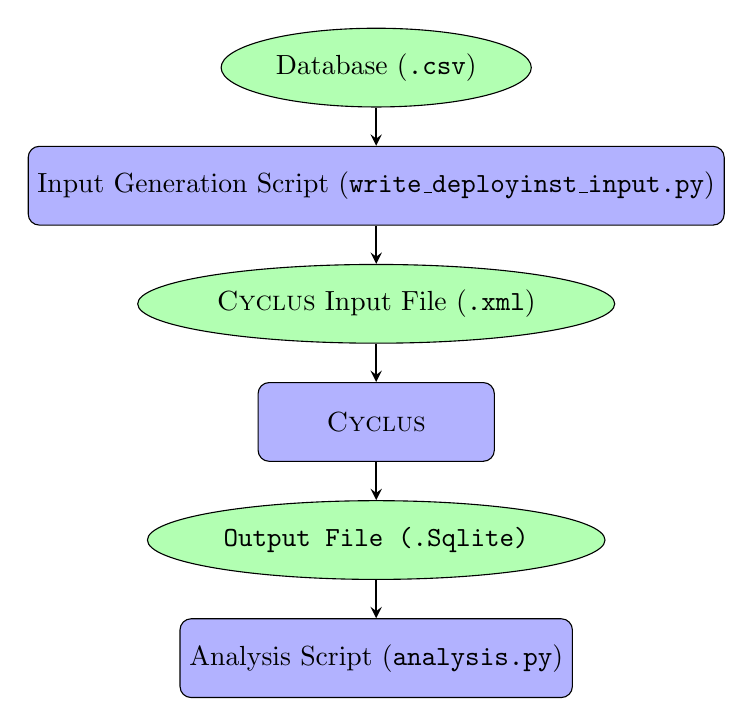
\begin{tikzpicture}[node distance=1.5cm]
\node (database) [object] {Database (\texttt{.csv})};
\node (script) [process, below of=database] {Input Generation Script (\texttt{write\_deployinst\_input.py})};
\node (input) [object, below of=script] {\Cyclus Input File (\texttt{.xml})};
\node (cyclus) [process, below of=input]{\Cyclus};
\node (output) [object, below of=cyclus]{\texttt{Output File (\texttt{.Sqlite})}};
\node (script2) [process, below of=output]{Analysis Script (\texttt{analysis.py})};

\draw [arrow] (database) -- (script); 
\draw [arrow] (script) -- (input); 
\draw [arrow] (input) -- (cyclus);
\draw [arrow] (cyclus) -- (output);
\draw [arrow] (output) -- (script2);
\end{tikzpicture}
}
\caption{Computational workflow in this work. The green circles represent files, and the blue
         boxes represent codes that process the files.}
\label{diag:comp}
\end{figure}


Projections of future reactor deployment in this simulation are based on
assessment of analyses from references such as \gls{PRIS} for reactors planned
for construction \cite{iaea_pris_2017}, the World Nuclear Association
\cite{world_nuclear_association_nuclear_2017}, and literature concerning the future of
nuclear power in a global \cite{joskow_future_2012} and European context
\cite{hatch_politics_2015}.  Existing projections extend to 2050.

\Cref{tab:eu_deployment} lists the reactors that are currently  planned or
under construction. In the simulation, all  planned constructions are completed 
without delay or failure and are assumed to reach a lifetime of 60 years.  

\begin{table}[h]
    \centering

    \label{tab:eu_deployment}
    \scalebox{0.9}{
    \begin{tabular}{ccccr}
        \hline
        \textbf{Exp. Operational }&\textbf{Country} &\textbf{Reactor} & \textbf{Type} & \textbf{Gross \gls{MWe}}\\
        \hline
        2018 & Slovakia  & Mochovce 3 & PWR & 440\\
        2018 & Slovakia & Mochovce 4 & PWR & 440 \\
        2018 & France & Flamanville 3 & PWR & 1600 \\
        2018 & Finland & Olkilouto 3 & PWR & 1720 \\
        2019 & Romania & Cernavoda 3 & PHWR & 720 \\
        2020 & Romania & Cernavoda 4 & PHWR & 720 \\
        2024 & Finland & Hanhikivi & VVER1200 & 1200 \\
        2024 & Hungary & Paks 5 & VVER1200 & 1200 \\
        2025 & Hungary & Paks 6 & VVER1200 & 1200 \\
        2025 & Bulgaria & Kozloduy 7 & AP1000? & 950 \\
        2026 & UK & Hinkley Point C1 & EPR & 1670 \\
        2027 & UK & Hinkley Point C2 & EPR & 1670 \\
        2029 & Poland & Choczewo & N/A & 3000 \\
        2035 & Poland & N/A & N/A & 3000 \\
        2035 & Czech Rep & Dukovany 5 & N/A & 1200 \\
        2035 & Czech Rep & Temelin 3 & AP1000 & 1200 \\
        2040 & Czech Rep & Temelin 4 & AP1000 & 1200 \\
        \hline
    \end{tabular}
    }
    \label{tab:eu_deployment}
    \caption {Power Reactors under construction and planned.
        Replicated from \cite{world_nuclear_association_nuclear_2017}.}
\end{table}
\FloatBarrier

For each \gls{EU} nation, we categorize the growth trajectory is categorized from
``Aggressive Growth'' to ``Aggressive Shutdown''. Aggressive growth is
characterized by a rigorous expansion of nuclear power while
Aggressive Shutdown is characterized as a transition to rapidly
de-nuclearize the nation's electric grid. A nation's growth trajectory is
categorized into five degrees depending on G, the growth trajectory metric.

 \[
 G = \left\{\begin{array}{ll}
 \text{Aggressive Growth}, & \text{for } G \geq 2\\
 \text{Modest Growth}, & \text{for } 1.2 \leq G < 2\\
 \text{Maintanence}, & \text{for } 0.8 \leq G < 1.2 \\
 \text{Modest Reduction}, & \text{for } 0.5 \leq G< 0.8\\
 \text{Aggressive Reduction}, & \text{for } G \leq 0.5
 \end{array}\right\} = \frac{C_{2040}}{C_{2017}}\\\\
 \]
 \[
  G = \text{Growth Trajectory  } [-] 
 \]
 \[
 C_{i} = \text{Nuclear Capacity in Year i  } [\gls{MWe}]
 \]

The growth trajectory and specific plan of each nation in the \gls{EU} 
is listed in Table \ref{tab:eu_growth}. Meanwhile, \cref{fig:eu_pow} displays the
timeseries of installed capacity in \gls{EU} nations.


\begin{table}[h]
    \centering
        \begin{tabular}{lll}
            \hline 
                    \textbf{Nation} & \textbf{Growth Trajectory} & \textbf{Specific Plan }\\
                    \hline
                    UK & Aggressive Growth & {\small  13 units (17,900 \gls{MWe}) by 2030.}\\
                    Poland & Aggressive Growth &  {\small Additional 6,000 \gls{MWe} by 2035.}\\
                    Hungary & Aggressive Growth &  {\small Additional 2,400 \gls{MWe} by 2025.} \\ 
                    Finland & Modest Growth &  {\small Additional 2,920 \gls{MWe} by 2024.}\\
                    Slovakia & Modest Growth & {\small Additional 942 \gls{MWe} by 2025.}\\
                    Bulgaria & Modest Growth &  {\small Additional 1,000 \gls{MWe} by 2035.} \\
                    Romania & Modest Growth &  {\small Additional 1,440 \gls{MWe} by 2020.} \\
                    Czech Rep. & Modest Growth & {\small  Additional 2,400 \gls{MWe} by 2035.}\\
                    France & Modest Reduction & {\small No expansion or early shutdown.}\\
                    Slovenia & Modest Reduction & {\small No expansion or early shutdown.}\\
                    Netherlands & Modest Reduction & {\small No expansion or early shutdown.}\\
                    Lithuania & Modest Reduction & {\small No expansion or early shutdown.}\\
                    Spain & Modest Reduction &  {\small No expansion or early shutdown.} \\
                    Italy & Modest Reduction & {\small No expansion or early shutdown. }\\
                    Belgium & Aggressive Reduction & All shut down 2025.\\
                    Sweden & Aggressive Reduction & All shut down 2050.\\
                    Germany & Aggressive Reduction & All shut down by 2022.\\
                    \hline
                    
        \end{tabular}

    \caption {Future Nuclear Programs of \gls{EU} Nations \cite{world_nuclear_association_nuclear_2017}}
  \label{tab:eu_growth}
\end{table}
\FloatBarrier

\begin{figure}[htbp!]
    \begin{center}
        \includegraphics[scale=0.6]{./images/eu_future/power_plot.png}
    \end{center}
    \caption{The timeseries of installed nuclear capacity in the EU is separated by \texttt{Region}s in \Cyclus.
             The sudden drops in capacity are caused by nuclear phaseout plans by nations such as Germany and Belgium.
             The extrapolations into the future are made
             }
    \label{fig:eu_pow}
\end{figure}


\subsection{French \gls{SFR} Deployment Schedule}

\Cref{fig:sfr_num} and \ref{fig:dep} display
the French transition to \glspl{SFR} modeled in this simulation.
Starting in 2040, France deploys 600-\gls{MWe} \glspl{SFR} to make up for 
decommissioned French \gls{LWR} capacity. This results in an installed 
\gls{SFR} 
capacity of 66,000 \gls{MWe} by 2078 when the final \gls{LWR} is 
decommissioned. 

\begin{figure}[htbp!]
        \begin{center}
                \includegraphics[scale=0.6]{./images/french-transition/power_plot.png}
        \end{center}
        \caption{This plot shows the potential French transition from \glspl{LWR} to \glspl{SFR}.
                 The aggressive growth of nuclear in the 1980s leads to a substantial shutdown
                 of nuclear in the 2040s, which, in the simulation, are replaced by new 
                 \glspl{SFR}. The net capacity is kept at a constant of 66 GWe.}
        \label{fig:sfr_num}
\end{figure}
\begin{figure}[htbp!]
    \begin{center}
        \includegraphics[scale=0.6]{./images/french-transition/sfr_deploy.png}
    \end{center}
    \caption{The deployment of \glspl{SFR} in France is characterized by a period of
             aggressive building. Four reactors on average are built per year to
             make up for the decommissioned power plants built in the 1980s and 1990s.
             The second period of aggressive building occurs when the first generation
             of \glspl{SFR} decommission after 80 years.}
    \label{fig:dep}
\end{figure}

\begin{figure}[htbp!]
    \begin{center}
        \includegraphics[scale=0.6]{./images/eu_future/onesim.png}
    \end{center}
    \caption{The total deployment scheme of the simulation. The historical
             operation \gls{EU} reactors is followed by the French
             transition to \glspl{SFR}.}
    \label{fig:tot_dep}
\end{figure}


\Cref{fig:tot_dep} displays the total deployment
scheme of the simulation.
The steep transition from 2040 to 2060 reflects the scheduled
decommissioning of reactors built in the 1975-2000
era of aggressive nuclear growth in France.

These figures reflect that, for the given assumptions, bursts of construction
are necessary to maintain capacity.  In reality, a construction rate of five 
reactors every year is highly unrealistic. However, this analysis is to analyze 
material flow, and demonstrates that, if such an aggressive deployment scheme 
took place, the \glspl{SFR} would have enough fuel.  More realistically, the 
deployment of new \glspl{SFR} can be spread out by staggering scheduled 
decommissioning of \glspl{LWR} through lifetime extensions.  An analysis of the 
effect of \gls{LWR} lifetime extension is discussed in Section \ref{sec:life}.

\subsection{Material Flow}

The fuel cycle is represented by a series of facility agents whose material 
flow is illustrated in figure \ref{diag:fc}, along with
the \Cyclus archetypes that were used to model each facility.

% Define block styles
\tikzstyle{decision} = [diamond, draw, fill=blue!20, 
text width=4.5em, text badly centered, node distance=3cm, inner sep=0pt]
\tikzstyle{block} = [rectangle, draw, fill=blue!20, 
text width=5em, text centered, rounded corners, minimum height=4em]
\tikzstyle{line} = [draw, -latex']
\tikzstyle{cloud} = [draw, ellipse,fill=red!20, node distance=3cm,
minimum height=2em]


\begin{figure}
        \centering
        \scalebox{0.6}{
                \begin{tikzpicture}[align=center, node distance = 3cm and 3cm, auto]
                % Place nodes
                \node [block] (sr) {Mine (\texttt{SOURCE})};
                \node [cloud, below of=sr] (nu) {Nat U};
                \node [block, below of=nu] (enr) {Enrichment ({\footnotesize \texttt{ENRICHMENT}})};
                \node [cloud, below of=enr] (uox) {\gls{UOX}};
                \node [block, below of=uox] (lwr) {\gls{LWR} (\texttt{REACTOR})};
                \node [cloud, right of=lwr] (snf) {\gls{UNF}};
                \node [cloud, right of=uox] (cunf) {Cooled \gls{UNF}};
                \node [block, right of=snf] (pool) {Pool (\texttt{Storage})};
                \node [cloud, left of=lwr] (tl2) {Dep U};
                \node [cloud, right of=enr] (tl) {Dep U};
                \node [block, right of=tl] (sk) {Repository (\texttt{SINK})};
                \node [cloud, below of=pool] (cunf2) {Cooled \gls{UNF}};
                \node [block, below of=snf] (rep) {{\small Reprocessing ({\footnotesize \texttt{SEPARATIONS}})}};
                \node [cloud, below of=rep] (u) {Sep. U} ;
                \node [cloud, left of=rep] (pu) {Sep. Pu};
                \node [block, left of=pu] (mix) {Fabrication (\texttt{MIXER})};
                \node [cloud, below of=mix] (mox) {\gls{MOX}};
                \node [block, below of=mox] (mxr) {\gls{MOX} Reactors};
                \node [cloud, right of= mxr] (snmox) {Spent \gls{MOX}};
                
                \draw[->, thick] (sr) -- (nu);
                \draw[->, thick] (nu) -- (enr);
                \draw[->, thick] (enr) -- (tl);
                \draw[->, thick] (enr) -- (tl2);
                \draw[->, thick] (tl) -- (sk);
                \draw[->, thick] (tl2) -- (mix);
                \draw[->, thick] (enr) -- (uox);
                \draw[->, thick] (uox) -- (lwr);
                \draw[->, thick] (lwr) -- (snf);
                
                \draw[->, thick] (lwr) -- (snf);
                \draw[->, thick] (snf) -- (pool);
                \draw[->, thick] (pool) -- (cunf);
                \draw[->, thick] (pool) -- (cunf2);
                \draw[->, thick] (cunf) -- (sk);
                \draw[->, thick] (cunf2) -- (rep);
                
                \draw[->, thick] (rep) -- (u);
                \draw[->, thick] (rep) -- (pu);
                \draw[->, thick] (pu) -- (mix);
                \draw[->, thick] (mix) -- (mox);
                \draw[->, thick] (mox) -- (mxr);
                \draw[->, thick] (mxr) -- (snmox);
                \draw[->, thick] (snmox) -- (rep);
                
                \end{tikzpicture}
        
                }
                \caption{The blue boxes represent fuel cycle facilities, and the red ovals
                         represent materials. The facility names in parenthesis are archetype names
                         used in \Cyclus. \gls{MOX} Reactors include both French \glspl{PWR} and
                         \glspl{SFR}.}
                \label{diag:fc}
\end{figure}

A mine facility provides natural uranium, which is enriched by an enrichment
facility to produce \gls{UOX}. Enrichment waste (tails) is disposed of to a 
sink facility representing ultimate disposal. The enriched \gls{UOX} fuels
the \glspl{LWR} which in turn produce spent \gls{UOX}. The used fuel
is sent to a wet storage facility to cool for at least 3 years \cite{carre_overview_2009}.

The cooled fuel is then reprocessed to separate plutonium and uranium,
or sent to the repository.
The plutonium mixed with depleted uranium (tails) makes \gls{MOX}.
Reprocessed uranium is unused and stockpiled. Uranium is reprocessed
in order to separate the raffinate (minor actinides and fission products)
from usable material. Though neglected in this work, reprocessed
uranium may substitute depleted uranium for \gls{MOX} production. In the
simulations, sufficient depleted uranium existed that using reprocessed
uranium was overlooked. However, further in the future where the depleted
uranium inventory drains, reprocessed uranium (or, natural uranium) will need to be utilized. 

\FloatBarrier

\section{Scenario Specifications}

The scenario specifications  are
listed in tables \ref{tab:gen}, \ref{tab:sim_eu}, and \ref{tab:sim_france}.
The reprocessing and \gls{MOX} fabrication capacity in France
prior to 2020 is modeled after the 
French La Hague and MELOX sites \cite{schneider_spent_2008, hugelmann_melox_1999}.


\begin{table}[h]
    \centering
    \begin{tabularx}{\textwidth}{bb}
        \hline
        \textbf{Specification} &\textbf{ Value} \\
        \hline
        Simulation Time & 1970-2160 \\ 
        Reprocessed Uranium Usage &  None. Stockpile reprocessed U \\
        Storage Residence Time & 36 months \\
        \gls{SFR} available year & 2040 \\
        Production of \gls{ASTRID} fuel begins & 2020 \\
        \hline
    \end{tabularx}
    \caption {General Simulation Specifications}
    \label{tab:gen}
\end{table}

\begin{table}[h]
    \centering
    \begin{tabularx}{\textwidth}{bb}
        \hline
        \textbf{Specification} &\textbf{ Value} \\
        \hline
        Reprocessing Capacity & 91.6 MTHM of \gls{UNF} per month \cite{schneider_spent_2008} \\
        Reprocessing Efficiency & 99.8\% \\
        Reprocessing Streams & plutonium and uranium \\
        \gls{MOX} Fabrication Throughput & 16.25 MTHM of \gls{MOX} per month  \cite{hugelmann_melox_1999} \\
        \gls{MOX} Fuel Reprocessing Stage &  Used \gls{MOX} is not reprocessed. \\  
        \hline
    \end{tabularx}
    \caption {Specification for Historical Operation of \gls{EU}}
    \label{tab:sim_eu}
\end{table}

\begin{table}[h]
    \centering
    \begin{tabularx}{\textwidth}{bb}
        \hline
        \textbf{Specification }& \textbf{Value} \\
        \hline
        Separation Efficiency & 99.8 \% \\
        Reprocessing Streams & plutonium and uranium \\
        \gls{ASTRID} Fuel Reprocessing Stage &  Used \gls{MOX} is reprocessed infinitely. \\
        \hline
    \end{tabularx}
    \caption {Specification for French Transition to \glspl{ASTRID} }
    \label{tab:sim_france}
\end{table}

\pagebreak

\section{Reactor Specifications}
Three major reactors are used in the simulation, \gls{PWR}, \gls{BWR}, and ASTRID-type \gls{SFR} reactors.


For \glspl{LWR}, we used a linear core size model to capture
varying reactor capacity. For example, a 
1,200 \gls{MWe} PWR has $193*\frac{1,200}{1,000} = 232$ \gls{UOX} assemblies, each
weighing 523.4 kg.
After each 18 month cycle, one-third of the 
core (77 assemblies) discharges. Refueling
is assumed to take two months to complete, during which the reactor
is shut down. The specifications are defined in 
table \ref{tab:reactor-specs} which details the reactor specifications in this simulation.

\begin{table}[h]
    \centering
    \begin{tabular}{cccc}
        \hline
        \textbf{Specification} & \textbf{\gls{PWR} \cite{sutharshan_ap1000tm_2011}} & \textbf{\gls{BWR} \cite{hinds_next-generation_2006}} & \textbf{\gls{SFR}} \cite{varaine_pre-conceptual_2012}\\
        \hline
                Lifetime [y] \tablefootnote{The simulated reactor lifetime reaches the licensed lifetime unless 
        the reactor is shut down prematurely.} & 60 & 60 & 80 \\
                Cycle Time [mos.]& 18 & 18 & 12\\ 
                Refueling Outage [mos.]& 2 & 2  & 2\\
                Rated Power [\gls{MWe}] & 1000 & 1000 & 600\\
                Assembly mass [kg] & 523.4 & 180 & -- \\
                Batch mass [kg] & -- & -- & 5,568\\
                Discharge Burnup [GWd/tHM] & 51 & 51 & 105 \\
                Assemblies per core \tablefootnote{Number of assemblies and corresponding \gls{LWR} core 
        masses are reported for a 1000-\gls{MWe} core. Reactors with different core  
        powers are modeled with a linear mass assumption.} & 193  & 764 & -- \\

                Batches per core & 3 & 3 & 4\\
        Initial Fissile Loading [t] & 3.1  $^{235}$U & 4.2  $^{235}$U & 4.9 Pu \\
                Fuel & \gls{UOX} or \gls{MOX} & \gls{UOX} & \gls{MOX} \\
        \hline
    \end{tabular}
        \caption {Model \gls{LWR} and \gls{ASTRID} specifications used for the simulations are listed, and \glspl{LWR} are modified
        linearly for varying power capacity. }
    \label{tab:reactor-specs}

    \end{table}


\subsection{Material Definitions}
Depletion calculations of the nuclear fuel are recipe-based, such that a fresh 
and used fuel recipe is defined for each reactor type.
For the compositions of the used fuel, a reference depletion calculation
from ORIGEN is used (see \cref{tab:comp}). ORIGEN is a computer code
system for calculating buildup, decay, and processing of radioactive materials
\cite{parks_overview_1992} The recipe has also been used for repository performance modeling \cite{wilson_adoption_2009}.

\begin{table}[h]
    \centering
%   \scalebox{0.86}{
        \begin{tabular}{cccc}
            \hline
             & \multicolumn{3}{c}{ Composition [\%]} \\
            Recipe & U-235  & U-238  & Pu \\ 
            \hline
            Fresh \gls{UOX} Fuel & 3.1 & 96.9 & -   \\ 
            Fresh \gls{MOX} Fuel & 0.2 & 90.7 & 9.1 \\ 
            Fresh \gls{ASTRID} Fuel & 0.2 & 77.7 & 22 \\
            \hline
        \end{tabular}
        \caption{Fresh fuel compositions used for the simulation \cite{wilson_adoption_2009, varaine_pre-conceptual_2012}.}
        \label{tab:sim_result}
\end {table}

\section{Results}

\subsection{Historical Operation of EU Reactors}


\begin{table}[h]
	\centering
	\scalebox{0.86}{
		\begin{tabular}{|c|c|c|}
			\hline
			Category [unit] & Value & Specifics \\ \hline
			Total UOX Usage [t] & 188,196  &  \\ \hline
			Total MOX Usage [t] & 118 & \\ \hline
			Total Spent UOX [t] & 183,807 & \\ \hline
			Total Spent MOX [t] & 0 & All is Reprocessed. \\ \hline
			Total Tailings [t] & 1,125,798 & \\ \hline
		\end{tabular}}
		\caption{Simulation Results}
		\label{tab:sim_result}
		\end {table}

Table \ref{tab:sim_result} lists the important metrics
obtained from the first simulation. The following
values are the EU inventory and history at year 2050.

Tables \ref{tab:eu_num} and \ref{tab:eu_pow} display the
timeseries of number of reactors and installed capacity in EU.



\begin{figure}[htbp!]
	\begin{center}
		\includegraphics[scale=0.7]{./images/eu_future/number_plot.png}
	\end{center}
	\caption{Timeseries of number of reactors in EU.}
	\label{fig:eu_num}
\end{figure}

\begin{figure}[htbp!]
	\begin{center}
		\includegraphics[scale=0.7]{./images/eu_future/power_plot.png}
	\end{center}
	\caption{Timeseries of installed nuclear capacity in EU.}
	\label{fig:eu_pow}
\end{figure}

Figures \ref{fig:eu_tail} and \ref{fig:snf} show the 
timeseries of mass of tailings and spent fuel accumulation in EU.

Figure \ref{fig:eu_fuel} shows the amount of fuel used in EU.
Note that the MOX usage is so little that it is invisible in the
plot. 


\begin{figure}[htbp!]
	\begin{center}
		\includegraphics[scale=0.7]{./images/eu_future/tailings.png}
	\end{center}
	\caption{Timeseries of Tailings in the EU.}
	\label{fig:eu_tail}
\end{figure}

\begin{figure}[htbp!]
	\begin{center}
		\includegraphics[scale=0.7]{./images/eu_future/total_fuel.png}
	\end{center}
	\caption{Timeseries of total fuel usage in EU.}
	\label{fig:eu_fuel}
\end{figure}


\begin{figure}[htbp!]
	\begin{center}
			\includegraphics[scale=0.7]{./images/eu_future/snf.png}
	\end{center}
	\caption{Timeseries of Spent Nuclear Fuel in Sink.}
	\label{fig:eu_snf}
\end{figure}

\begin{table}[h]
	\centering
	\begin{tabular}{|c|c|c|}
		\hline
		Isotope & Mass Fraction in Spent Fuel [\%] & Quantity [t] \\ \hline
		Total & .9358 & 1,720 \\ \hline
		Pu238 & .0111 & 20.40 \\ \hline
		Pu239 & .518 & 952.12 \\ \hline
		Pu240 & .232 & 426.43 \\ \hline
		Pu241 & .126 & 231.59 \\ \hline
		Pu242 & .0487 & 89.51 \\ \hline
	\end{tabular}
	\caption{Plutonium From Spent Fuel}
	\label{tab:pu}
\end{table}


To create \gls{MOX}, 10\% Pu and 90\% depleted uranium is used.
Thus $1,720$ tons of plutonium yields $17,200$ tons of
\gls{MOX}. Table \ref{tab:pu} lists the isotope, mass fraction,
and quantity of plutonium that can be obtained from the 2050 \gls{SNF} inventory.


\subsection{French \gls{SFR} Transition Scenario}

From Varaine et al \cite{marsaultmarie-sophie_pre-conceptual_2012}, a French
ASTRID-type \gls{SFR} of capacity $600 MWe$ needs $1.225$ tons of
plutonium a year, with an initial plutonium loading of $4.9$ tons.
Thus, it can be assumed that the ASTRID reactor takes in $49$ tons of 
\gls{MOX}, and refuels a quarter of its fuel every year. Simply,
an ASTRID reactor needs $12.25$ tons of \gls{MOX} per year. 

The number of SFR-years worth of fuel that can be created with
the \gls{SNF} from 2050 is $\frac{17,611.3 t}{12.25} = 1,437.65 $,
assuming infinite reprocessing and \gls{MOX} fabrication capacity.

However, assuming that \gls{MOX} can be recycled indefinitely,
spent \gls{MOX} from an ASTRID reactor
contains enough plutonium to produce a \gls{MOX} fuel with
the same mass, if mixed with depleted uranium. For example,
spent \gls{MOX} from an ASTRID reactor is 38\% plutonium,
whereas a fresh \gls{MOX} is 10\% plutonium.
The compositions are in appendix table \ref{tab:comp}.
Separating plutonium from spent \gls{MOX} from
an ASTRID reactor can create \gls{MOX} more than
three times the mass of spent \gls{MOX}.

The second scenario, with the tails and spent \gls{UOX}
inventory, evaluates if the French can transition into \gls{SFR}
without constructing additional \gls{LWR}s. This simulation
assumed infinite reprocessing and fabrication capacity.

Figure \ref{fig:fuel} shows the mass of \gls{MOX} used in the 
\gls{SFR}s separated by how they are made, over time.
Note that the mass of \gls{MOX} from the spent \gls{UOX}
stops increasing around 2050, which means that the spent
\gls{MOX} is enough to create the \gls{MOX} for the
\gls{SFR} fleet. 

\begin{figure}[htbp!]
	\begin{center}
		\includegraphics[scale=0.7]{./images/french-transition/where_fuel.png}
	\end{center}
	\caption{Timeseries of fuel used in the \gls{SFR}s [tons]}
	\label{fig:fuel}
\end{figure}

Figure \ref{fig:mox_fab} shows the progression of mox created from
the fabrication plant over time. Figure \ref{fig:mox_fab} shows
the separated plutonium demand from spent \gls{MOX} to fuel the 
ASTRID reactors.

Figure \ref{fig:reprocess_waste} shows the amount of reprocessing waste
(any content from spent fuel other than U, Pu) over time. Note that 
the amount of reprocessing waste is much greater when reprocessing
spent \gls{MOX} from ASTRID reactors, since there is little uranium
or plutonium left due to a high burnup.

\begin{figure}[htbp!]
	\begin{center}
		\includegraphics[scale=0.7]{./images/french-transition/mox_from_mixer.png}
	\end{center}
	\caption{Timeseries of MOX produced from Fabrications}
	\label{fig:mox_fab}
\end{figure}


\begin{figure}[htbp!]
	\begin{center}
		\includegraphics[scale=0.7]{./images/french-transition/pu_demand.png}
	\end{center}
	\caption{Separated Plutonium demand from Spent MOX}
	\label{fig:pu_demand_mox}
\end{figure}

\begin{figure}[htbp!]
	\begin{center}
		\includegraphics[scale=0.7]{./images/french-transition/reprocess_waste.png}
	\end{center}
	\caption{Reprocessing Waste for French Transition Scenario.}
	\label{fig:reprocess_waste}
\end{figure}


\begin{table}[h]
	\centering
	\scalebox{0.86}{
		\begin{tabular}{|c|c|c|}
			\hline
			Category [unit] & Value & Specifics \\ \hline
			Total MOX used [t] & 164,141 & \\ \hline
			Total MOX from UOX Waste [t] & 2,347.2  &  \\ \hline
			Total MOX from MOX Waste [t] & 161,793.8 & \\ \hline
		\end{tabular}}
		\caption {\gls{SFR} Simulation Results}
		\label{tab:sfr_sim_result}
\end {table}



\section{Conclusion}

This work demonstrates that France can transition into
a fully \gls{SFR} fleet with installed capacity of 66,000 MWe without
building additional \glspl{LWR}
if France receives \gls{UNF} from other \gls{EU} nations.
Supporting the \gls{SFR} fleet would require a reprocessing capacity of 250 MTHM per month,
and a fabrication capacity of 200 MTHM per month.


Since most \gls{EU} nations do not have an operating \gls{UNF}
repository or a management plan, they have a strong incentive
to send all their \gls{UNF} to France. The nations
with aggressive nuclear reduction will be able phase out nuclear
without constructing a permanent repository. France has an
incentive to take this fuel, since recycling of used fuel from
other nations will allow France to meet their MOX demand
without new construction of \glspl{LWR}.

\Cref{tab:which_send} proposes a strategy where nations
that are planning a nuclear phaseout send their \gls{UNF}
to France. The sum of \gls{UNF} from the four countries
provide enough \gls{UNF} for the simulated transition.
The four nations would then be able to decommission
their reactors without building a permanent repository. 

\begin{table}[h]
    \centering
                \begin{tabularx}{\textwidth}{lbb}
                       \hline 
                    
                    \textbf{Nation} & \textbf{Growth Trajectory} & \small{\textbf{UNF in 2050 [MTHM] }}\\
                    \hline
                    UK & Aggressive Growth & 53,188\\
                    \hline
                    Poland & Aggressive Growth & 6,714\\
                    \hline
                    Hungary & Aggressive Growth & 4,768 \\ 
                    \hline
                    Finland & Modest Growth &  7,528\\
                    \hline
                    Slovakia & Modest Growth & 3,446\\
                    \hline
                    Bulgaria & Modest Growth & 3,930 \\
                    \hline
                    Czech Rep. & Modest Growth & 7,583\\
                    \hline
                    Slovenia & Modest Reduction & 765\\
                    \hline
                    Netherlands & Modest Reduction & 539\\
                    \hline
                    Lithuania & Modest Reduction & 2,644 \\
                    \hline
                    \textbf{France} & \textbf{Modest Reduction} & \textbf{12,943} \\
                    \hline 
                    \textbf{Spain} & \textbf{Modest Reduction} &  \textbf{9,771} \\
                    \hline
                    \textbf{Italy} & \textbf{Modest Reduction} & \textbf{583}\\
                    \hline
                    \textbf{Belgium} & \textbf{Aggressive Reduction} & \textbf{6,644}\\
                    \hline
                    Sweden & Aggressive Reduction & 16,035\\
                    \hline
                    \textbf{Germany} & \textbf{Aggressive Reduction} & \textbf{23,868}\\
                    \hline
                \end{tabularx}
    \caption {\gls{EU} nations and their respective \gls{UNF} inventory. The bolded countries'
              \gls{UNF} inventory adds up to the required \gls{UNF} amount for French \gls{SFR} transition. }
    \label{tab:which_send}

\end{table}

Though complex political and economic factors are overlooked,
 and various assumptions present for this scenario,
this option may hold value for the \gls{EU} as a nuclear community,
and for France to advance into a closed fuel cycle.

\section{Acknowledgment}

The authors would like to thank the members of Advanced Reactors and
Fuel Cycles research group (ARFC) at the University
of Illinois - Urbana Champaign, namely Gyu-Tae Park for code
reviews and proofreading of the paper.


\bibliography{bibliography}

% Prof. Huff discourages appendices in journal articles.
% But, if you must, include one like so:
%\pagebreak
%\section{Fresh and Used Fuel Composition}
\begin{table}[h]
	\centering
	\scalebox{0.75}{
		\begin{tabular}{|c|c|c|c|c|c|c|}
		\hline
		 Isotope 	 & 	Fresh UOX Fuel & 	Spent UOX Fuel (BU: $51\frac{GWdth}{MTHM}$) & Fresh SFR Fuel & Spent SFR Fuel \\ \hline 
		 He4	 & 	 	& 	9.474E-07 & 	 	 & 	7.827E-06 \\ \hline 
		 Ra226	 & 	 	& 	9.788E-14 & 	 	 & 	5.151E-14 \\ \hline 
		 Ra228	 & 	 	& 	2.750E-20 & 	 	 & 	4.904E-21 \\ \hline 
		 Pb206	 & 	 	& 	5.574E-18 & 	 	 & 	1.210E-18 \\ \hline 
		 Pb207	 & 	 	& 	1.685E-15 & 	 	 & 	1.892E-16 \\ \hline 
		 Pb208	 & 	 	& 	3.688E-12 & 	 	 & 	5.875E-11 \\ \hline 
		 Pb210	 & 	 	& 	3.023E-19 & 	 	 & 	8.143E-18 \\ \hline 
		 Th228	 & 	 	& 	8.475E-12 & 	 	 & 	1.004E-10 \\ \hline 
		 Th229	 & 	 	& 	2.727E-12 & 	 	 & 	4.065E-12 \\ \hline 
		 Th230	 & 	 	& 	2.625E-09 & 	 	 & 	2.139E-09 \\ \hline 
		 Th232	 & 	 	& 	4.174E-10 & 	 	 & 	4.425E-11 \\ \hline 
		 Bi209	 & 	 	& 	6.607E-16 & 	 	 & 	2.600E-14 \\ \hline 
		 Ac227	 & 	 	& 	3.096E-14 & 	 	 & 	4.840E-15 \\ \hline 
		 Pa231	 & 	 	& 	9.246E-10 & 	 	 & 	1.300E-10 \\ \hline 
		 U232	 & 	 	& 	0.000 & 	 	 & 	0.000 \\ \hline 
		 U233	 & 	 	& 	2.213E-09 & 	 	 & 	5.528E-09 \\ \hline 
		 U234	 & 	0.000& 	0.000 & 	 	 & 	0.000 \\ \hline 
		 U235	 & 	0.032& 	0.007 & 	0.002 & 	0.000 \\ \hline 
		 U236	 & 	 	& 	0.005 & 	 	 & 	0.000 \\ \hline 
		 U238	 & 	0.968& 	0.920 & 	0.887 & 	0.808 \\ \hline 
		 Np237	 & 	 	& 	0.000 & 	 	 & 	0.000 \\ \hline 
		 Pu238	 & 	 	& 	0.000 & 	0.001 & 	0.001 \\ \hline 
		 Pu239	 & 	 	& 	0.006 & 	0.060 & 	0.085 \\ \hline 
		 Pu240	 & 	 	& 	0.002 & 	0.027 & 	0.027 \\ \hline 
		 Pu241	 & 	 	& 	0.001 & 	0.014 & 	0.003 \\ \hline 
		 Pu242	 & 	 	& 	0.000 & 	0.005 & 	0.001 \\ \hline 
		 Pu244	 & 	 	& 	2.864E-08 & 1.508E-07 & 	5.461E-09 \\ \hline 
		 Am241	 & 	 	& 	6.442E-05 & 	 	 & 	0.001 \\ \hline 
		 Am242m	 & 	 	& 	8.533E-07 & 	 	 & 	7.961E-05 \\ \hline 
		 Am243	 & 	 	& 	0.000 & 	 	 & 	0.000 \\ \hline 
		 Cm242	 & 	 	& 	2.589E-05 & 	 	 & 	5.331E-05 \\ \hline 
		 Cm243	 & 	 	& 	0.000 & 	 	 & 	3.242E-06 \\ \hline 
		 Cm244	 & 	 	& 	8.561E-05 & 	 	 & 	0.000 \\ \hline 
		 Cm245	 & 	 	& 	5.721E-06 & 	 	 & 	3.936E-05 \\ \hline 
		 Cm246	 & 	 	& 	7.295E-07 & 	 	 & 	1.434E-05 \\ \hline 
		 Cm247	 & 	 	& 	0.000 & 	 	 & 	5.317E-07 \\ \hline 
		 Cm248	 & 	 	& 	7.691E-10 & 	 	 & 	0.000 \\ \hline 
		 Cm250	 & 	 	& 	4.280E-18 & 	 	 & 	6.407E-15 \\ \hline 
		 Cf249	 & 	 	& 	1.649E-12 & 	 	 & 	6.446E-10 \\ \hline 
		 Cf250	 & 	 	& 	2.041E-12 & 	 	 & 	6.703E-11 \\ \hline 
		 Cf251	 & 	 	& 	9.865E-13 & 	 	 & 	1.903E-12 \\ \hline 
		 Cf 252	 & 	 	& 	6.579E-13 & 	 	 & 	4.014E-14 \\ \hline 
		 H3	 & 	 	& 	8.584E-08 & 	 	 & 	1.747E-07 \\ \hline 
		 C14	 & 	 	& 	4.057E-11 & 	 	 & 	 	 \\ \hline 
		 C Other	 & 	 	& 	 	 & 	 	 & 	 	 \\ \hline 
		 Kr81	 & 	 	& 	4.216E-11 & 	 	 & 	8.038E-12 \\ \hline 
		 Kr85	 & 	 	& 	3.444E-05 & 	 	 & 	2.950E-05 \\ \hline 
		 Kr Other	 & 	 	& 	0.000 & 	 	 & 	0.000 \\ \hline 
		 Sr90	 & 	 	& 	0.001 & 	 	 & 	0.001 \\ \hline 
		 Sr Other	 & 	 	& 	0.000 & 	 	 & 	0.000 \\ \hline 
		 Tc99	 & 	 	& 	0.000 & 	 	 & 	5.391E-05 \\ \hline 
		 Tc Other	 & 	 	& 	0.000 & 	 	 & 	0.002 \\ \hline 

		\end{tabular}}
		\caption{Fresh and Spent Fuel Compositions}
		\label{tab:comp}
\end {table}


\end{document}
